
% !TeX root = ./slides-13.tex

\setcounter{section}{12}

\section{Further topics}

\subsection{History of logic}

\begin{frame}
  \frametitle{The beginnings}
  \begin{columns}
    \begin{column}{.5\textwidth}
    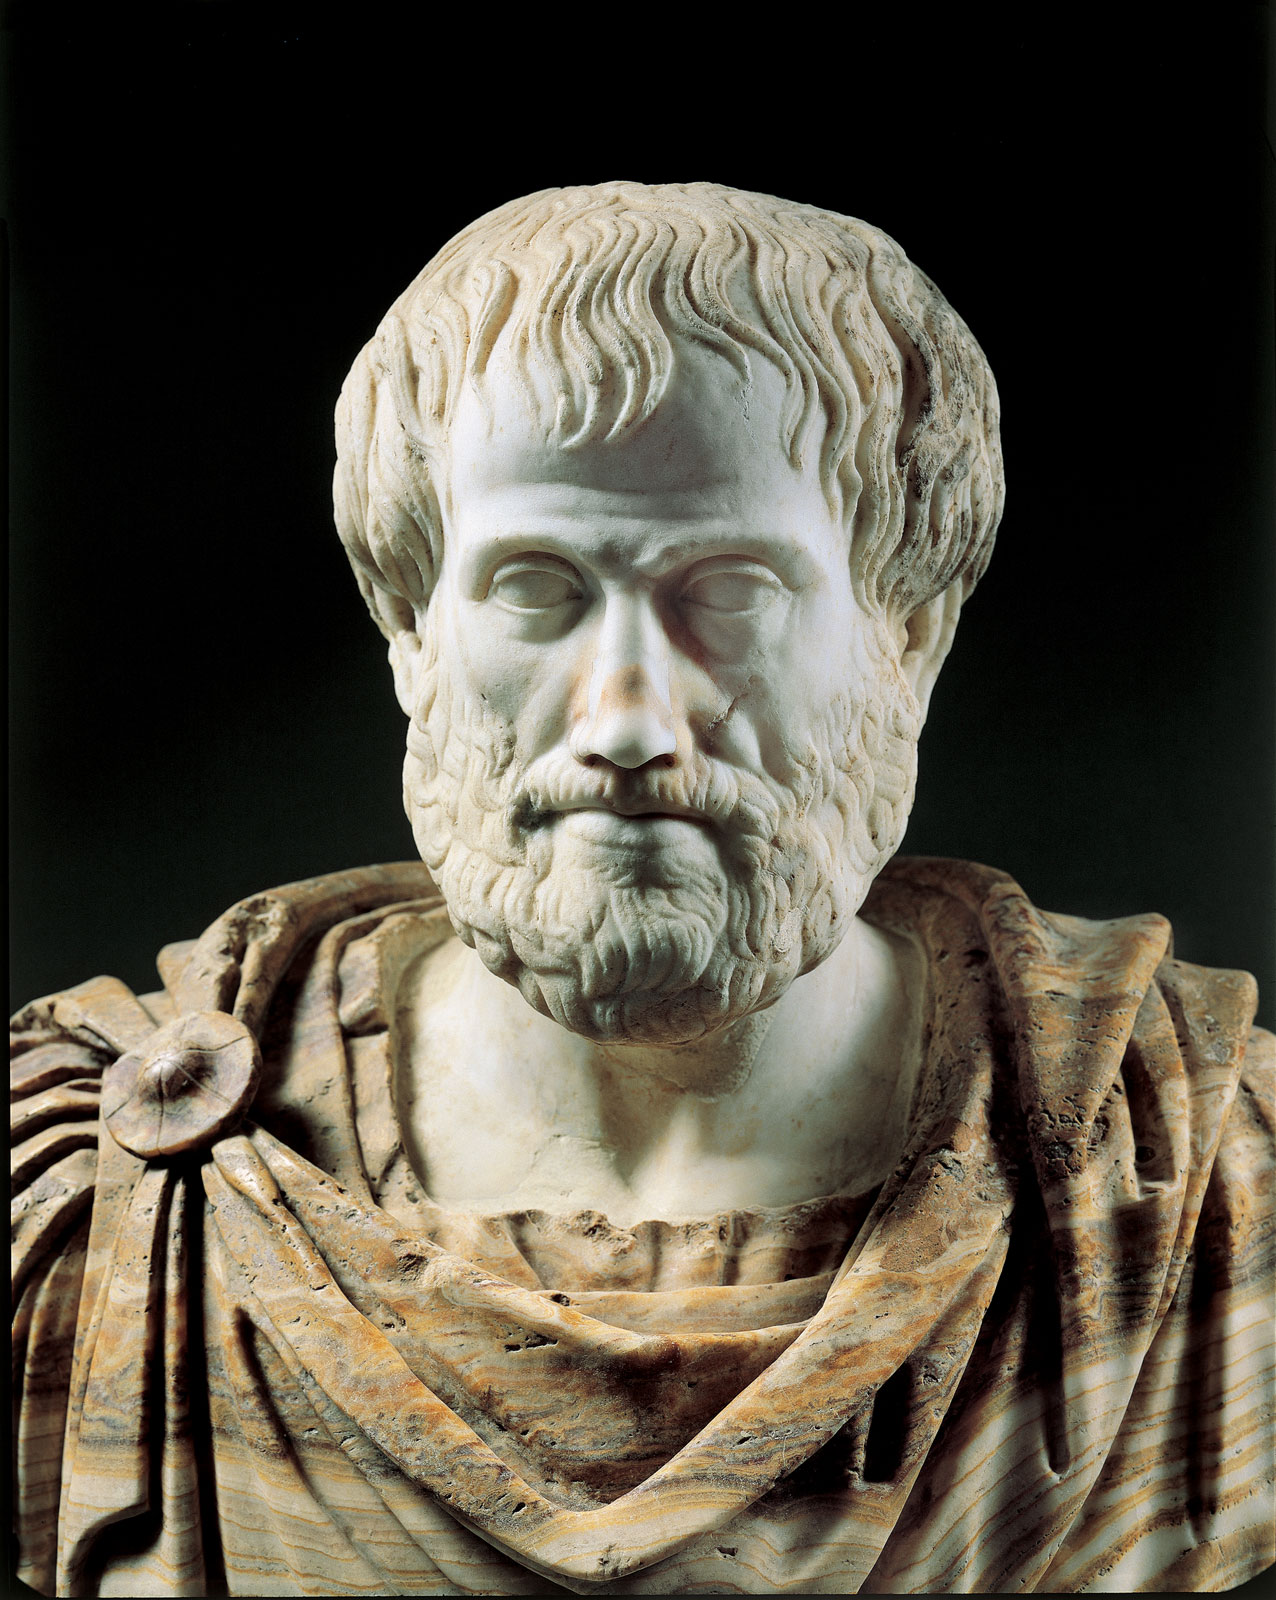
\includegraphics[height=.8\textheight]{../assets/aristotle}
    \end{column}
    \begin{column}{.5\textwidth}
      \begin{itemize}[<+->]
        \item Rules of debate \& rhetoric
        \item Ancient India: Gautama, \emph{Nyayasutra} (600 BCE-200
        CE)
        \item Ancient Greece: Aristotle (384--322 BCE)
        \item Cataloged valid arguments (``syllogisms''), e.g.,
        \item All ungulates have hooves.\\
        No fish have hooves.\\
        $\therefore$ No fish are ungulates.
      \end{itemize}
    \end{column}
  \end{columns}
\end{frame}

\begin{frame}
  \frametitle{The middle ages}
  \begin{columns}
    \begin{column}{.5\textwidth}
    
\includegraphics[height=.8\textheight]{../assets/avicenna}
    \end{column}
    \begin{column}{.5\textwidth}
      \begin{itemize}[<+->]
        \item Ibn S\=\i n\=a (Avicenna)
        \item Pierre Abelard
        \item William Ockham
        \item Jean Buridan
      \end{itemize}
    \end{column}
  \end{columns}
\end{frame}

\begin{frame}
  \frametitle{Mathematical logic}

  \begin{columns}
    \begin{column}{.5\textwidth}
    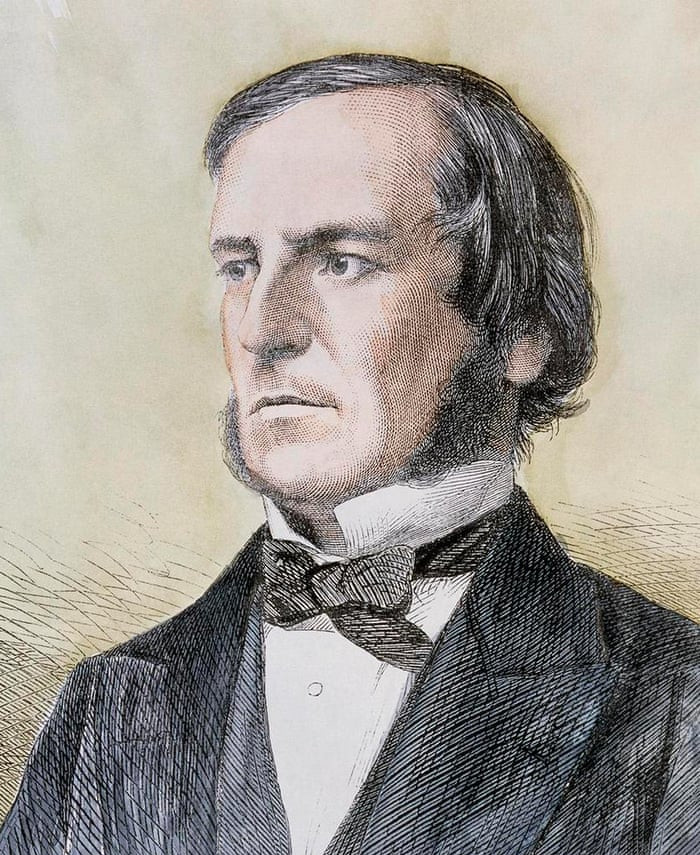
\includegraphics[height=.8\textheight]{../assets/boole}
    \end{column}
    \begin{column}{.5\textwidth}
      \begin{itemize}[<+->]
        \item George Boole
        \item John Venn
        \item Augustus De Morgan
        \item Charles Lutwidge Dodgson (aka Lewis Caroll)
      \end{itemize}
    \end{column}
  \end{columns}
\end{frame}

\begin{frame}
  \frametitle{Modern logic: Peirce at al}

  \begin{columns}
    \begin{column}{.5\textwidth}
      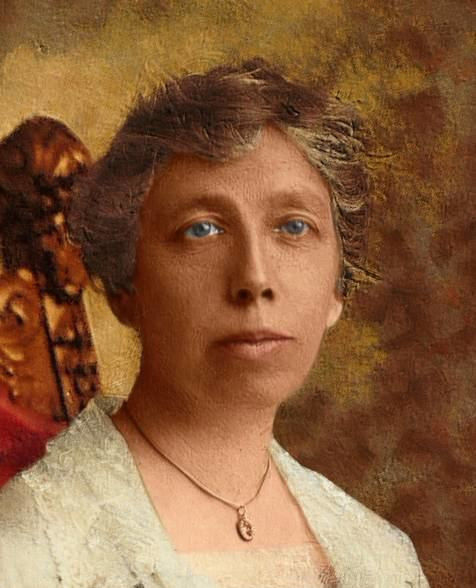
\includegraphics[height=.8\textheight]{../assets/ladd-franklin}
    \end{column}
    \begin{column}{.5\textwidth}
      \begin{itemize}[<+->]
        \item Charles Sanders Peirce
        \item Christine Ladd Franklin
        \item Ernst Schr\"oder
      \end{itemize}
    \end{column}
  \end{columns}
\end{frame}

\begin{frame}
  \frametitle{Modern logic: Gottlob Frege}

  \begin{columns}
    \begin{column}{.5\textwidth}
      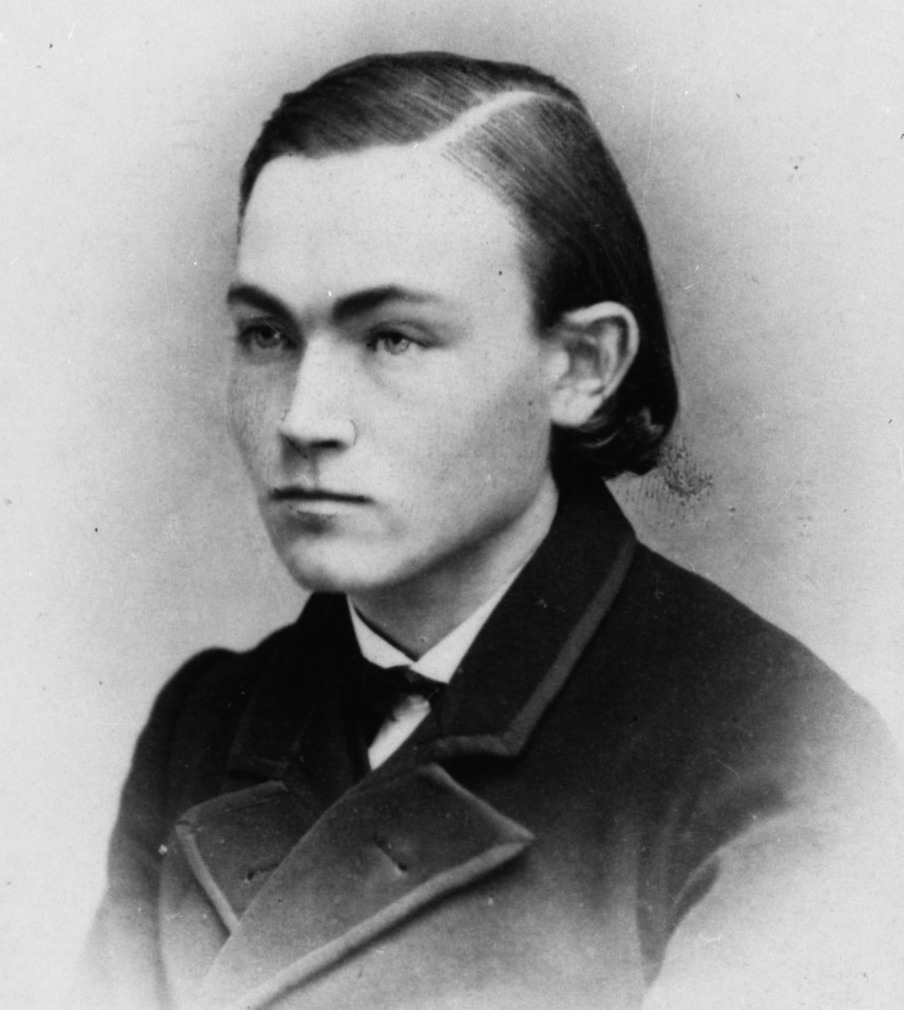
\includegraphics[height=.8\textheight]{../assets/frege}
    \end{column}
    \begin{column}{.5\textwidth}
      \begin{itemize}[<+->]
        \item 1848--1925
        \item Predicates and quantifiers
        \item Plan to turn all of math into theorems of logic alone
      \end{itemize}
    \end{column}
  \end{columns}
\end{frame}

\begin{frame}
  \frametitle{Modern logic: Bertrand Russell}

  \begin{columns}
    \begin{column}{.5\textwidth}
      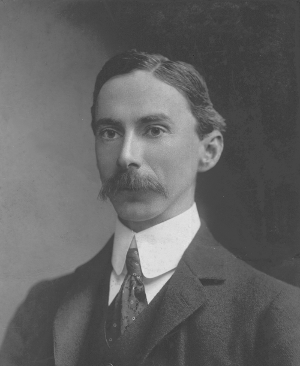
\includegraphics[height=.8\textheight]{../assets/russell}
    \end{column}
    \begin{column}{.5\textwidth}
      \begin{itemize}[<+->]
        \item 1870--1972
        \item Showed Frege's system contradictory (1902)
        \item Fixed it (\textit{Principia mathematica} 1910--13, 3 vols.)
        \item Plan to turn all of math into theorems of logic alone
      \end{itemize}
    \end{column}
  \end{columns}
\end{frame}

\begin{frame}
  \frametitle{Modern logic: David Hilbert}

  \begin{columns}
    \begin{column}{.5\textwidth}
      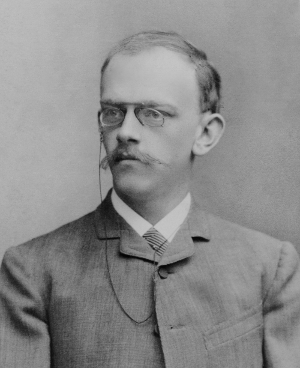
\includegraphics[height=.8\textheight]{../assets/hilbert}
    \end{column}
    \begin{column}{.5\textwidth}
      \begin{itemize}[<+->]
        \item 1862--1943
        \item Combined Russell's and Schr\"oder's systems
        \item First modern logic textbook
        \item Plan to turn all of math into consequences of a single set of premises
      \end{itemize}
    \end{column}
  \end{columns}
\end{frame}

\begin{frame}
  \frametitle{Modern logic: Kurt G\"odel}

  \begin{columns}
    \begin{column}{.5\textwidth}
      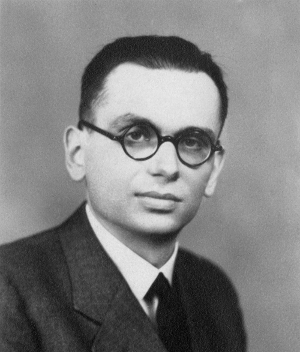
\includegraphics[height=.8\textheight]{../assets/goedel}
    \end{column}
    \begin{column}{.5\textwidth}
      \begin{itemize}[<+->]
        \item 1906--1978
        \item Showed that every valid argument has a proof
        \item Showed that Frege/Russell's and Hilbert's plans can't work
      \end{itemize}
    \end{column}
  \end{columns}
\end{frame}

\begin{frame}
  \frametitle{Modern logic: Alan Turing}

  \begin{columns}
    \begin{column}{.5\textwidth}
      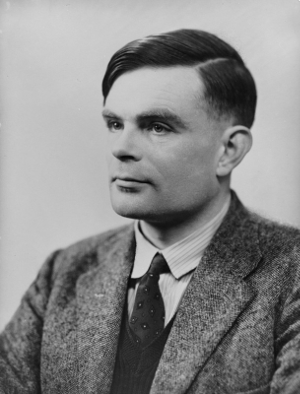
\includegraphics[height=.8\textheight]{../assets/turing}
    \end{column}
    \begin{column}{.5\textwidth}
      \begin{itemize}[<+->]
        \item 1912--1954
        \item Showed that unlike SL, QL has no decision procedure
        \item Invented Turing machines (``father of computer science'')
      \end{itemize}
    \end{column}
  \end{columns}
\end{frame}

\begin{frame}
  \frametitle{Modern logic: Gerhard Gentzen}

  \begin{columns}
    \begin{column}{.5\textwidth}
      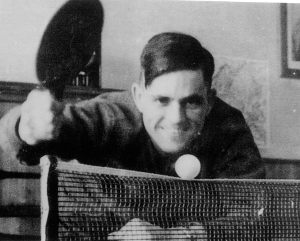
\includegraphics[width=\textwidth]{../assets/gentzen}
    \end{column}
    \begin{column}{.5\textwidth}
      \begin{itemize}[<+->]
        \item 1909--1945
        \item Invented natural deduction
        \item Founded theory of proofs
      \end{itemize}
    \end{column}
  \end{columns}
\end{frame}

\begin{frame}
  \frametitle{Modern logic: modal logic}

  \begin{columns}
    \begin{column}{.5\textwidth}
      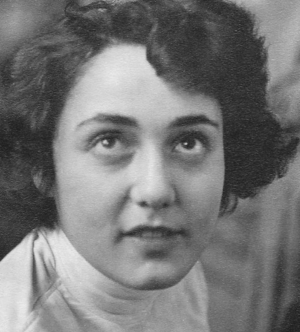
\includegraphics[height=.8\textheight]{../assets/barcan}
    \end{column}
    \begin{column}{.5\textwidth}
      \begin{itemize}[<+->]
        \item Extend logic with operators for ``possible'' and ``necessary''
        \item Pioneered by philosophers, now used by computer scientists
        \item Rudolf Carnap, Saul Kripke, Ruth Barcan Marcus
      \end{itemize}
    \end{column}
  \end{columns}
\end{frame}

\subsection{Philosophy and nonstandard logics}

\begin{frame}
    \frametitle{Validity and validity in QL}

\begin{itemize}[<+->]
\item Philosophers interested in \emph{valid arguments}
\item Definition: There is no case where the
premises are true and the conclusion is false
\begin{itemize}[<+->]
\item \emph{Important:} It does not say ``it \emph{isn't in fact the case} that the premises
are true and the conclusion is false''
\item That would make every argument with
\begin{itemize}[]
\item true premises, true conclusion
\item false premises, true conclusion
\item false premises, false conclusion
\end{itemize}
valid.  But that's not the case.
\item It says ``it is \emph{impossible} that the premises could be true and the conclusion false!''
\end{itemize}
\item Difficulty: What logically possible circumstances are there?
\end{itemize}

\end{frame}

\begin{frame}
    \frametitle{What logic does for validity}

\begin{itemize}[<+->]
\item Truth-tables, interpretations, proofs give \emph{sufficient conditions}
for validity, i.e.,
\begin{itemize}
\item Every argument valid in SL is valid
\item Every argument valid in QL is valid
\item Every argument with a formal proof is valid (soundness!)
\end{itemize}
\end{itemize}

\end{frame}

\begin{frame}
    \frametitle{Nonstandard logics}

\begin{itemize}[<+->]
\item Formal models of logical consequence make a number of simplifying assumptions:
\begin{itemize}[<+->]
\item Only \emph{determinate} properties allowed, e.g, no vague properties
\item Every (atomic) sentence either \True{} or \False; not both and nothing in between
\item Every name must refer, i.e., no empty names
\item Only truth-functional connectives, e.g., no subjunctive contionals, ``because'', or tenses
\end{itemize}
\item Non-standard logics: expand SL, QL to deal with these
\end{itemize}

\end{frame}

\begin{frame}
    \frametitle{Many-valued logic}
\def\I{\textcolor{highlightA}{\textbf{U}}}
\begin{itemize}
\item Add to the truth-values \True{} and \False, e.g.,
\begin{itemize}
\item ``Undetermined'': neither true nor false
\[
\begin{array}{c|c}
P & \lnot P\\
\hline
\True & \False \\
\I & \I\\
\False & \True
\end{array}
\qquad
\begin{array}{cc|c}
P & Q & (P \land Q)\\
\hline
\True & \True & \True\\
\True & \I & \I\\
\True & \False & \False\\
\I & \True & \I\\
\I & \I & \I\\
\I & \False & \False\\
\False & \True & \False\\
\False & \I & \False\\
\False & \False & \False
\end{array}
\qquad
\begin{array}{cc|c}
P & Q & (P \lor Q)\\
\hline
\True & \True & \True\\
\True & \I & \True\\
\True & \False & \True\\
\I & \True & \True\\
\I & \I & \I\\
\I & \False & \I\\
\False & \True & \True\\
\False & \I & \I\\
\False & \False & \False
\end{array}
\]
\item ``Inconsistent'': both true and false
\item Fuzzy truth values: any number between 0 and 1
\end{itemize}
\end{itemize}

\end{frame}

%\subsection{Truth-functionality}

\begin{frame}
\frametitle{Truth-functional connectives}

\begin{block}{Definition}
  A connective $*$ is \emph{truth functional} iff the truth value of $*A$ depends only on the truth value of $A$.
\end{block}

\begin{itemize}[<+->]
  \item ``It is not the case that'' is truth functional.
  \item So are ``and'', ``or'', ``neither nor''.
  \item ``If \dots then'': iffy.
\end{itemize}

\end{frame}


\begin{frame}
  \frametitle{Non-truth-functional connectives}
  
  \begin{itemize}[<+->]
    \item ``Possibly'', ``Necessarily''
    \item Subjunctive conditionals
    \item Tenses: ``Is always true,'' ``Will be true,'' ``Was true''
    \item ``Richard believes that'', ``Richard knows that''
  \end{itemize}
  \end{frame}
  
\begin{frame}
\frametitle{Possibly}

  \begin{itemize}[<+->]
    \item ``It is possible that \dots'', ``Possibly, \dots''
    \item Consider:
      \begin{enumerate}[<+->]
        \item It is possible that I will live forever.
        \item It is possible that $2+2=5$.
      \end{enumerate}
    \item (1) is true and (2) is false.
    \item But $A_1=$ ``I will live forever'' and
    $A_2=$ ``$2+2=5$'' are both false.
    \item So ``It is possible that $A$'' can't just depend on the
    truth value of $A$
    \item Otherwise (1) and (2) would have to have the same truth value.
  \end{itemize}

\end{frame}

\begin{frame}
\frametitle{Subjunctive Conditionals}

\begin{itemize}[<+->]
\item Subjunctive conditionals = if---then statements in \emph{subjunctive} mood
\item ``If P were true, then Q would be true.''
\item Indicative conditional is (plausibly) \emph{truth-functional}:
  truth value of ``If P, then Q'' depends \emph{only on truth values}
  of P and Q.
\end{itemize}
\end{frame}

\begin{frame}
\frametitle{Subjunctive Conditionals}

\begin{itemize}[<+->]
\item Subjunctive conditional is not truth functional
\item E.g., consider:
\begin{enumerate}
\item If the world were just, no evil deed would go unpunished.\\
$P_1$ = the world is just\\
$Q_1$ = no evil deed goes unpunished
\item If the world were flat, no evil deed would go unpunished.\\
$P_2$ = the world is flat\\
$Q_2$ = no evil deed goes unpunished
\end{enumerate}
\item $P_1$, $Q_1$ both false; $P_2$, $Q_2$ both false, but
\item (1) is true, but (2) is false
\end{itemize}
\end{frame}

\begin{frame}
    \frametitle{Modal logic}

\begin{itemize}[<+->]
\item Alethic logic: 
``It is possible that'' ($\Diamond$), ``it is necessary that'' ($\Box$)
\[
\Box A \to A \qquad \Diamond\Box A \to \Box A
\]
\item Epistemic logic:
``Richard knows that'' (K)
\[
\textbf{K}\, A \to A \qquad \textbf{K} A \to \textbf{K}\textbf{K}\, A
\]
\item Conditional logic\\
Subjunctive conditionals, ``if it were true that \dots, then it would be true that --- ---'' ($\Box\!\!\to$)
\[
(A \mathrel{\Box\!\!\to} B) \to (A \to B)
\]
\item Temporal logic\\
``It was true that'' (P), ``It will be true that'' (F)
\[
\textbf{F}\,\textbf{P}\, A \to (\textbf{P}\, A \lor A \lor \textbf{F}\, A)
\]
\end{itemize}

\end{frame}

\begin{frame}
\frametitle{Temporal logic}

\begin{itemize}[<+->]
  \item ``Always $A$'': $\Box A$
  \item ``Sometimes $A$'': $\Diamond A$
  \item If always $A$, then $A$ (now): $\Box A \to A$
  \item If $A$ (now), then sometimes $A$: $A \to \Diamond A$
  \item Always $A$ iff not sometimes not~$A$\\
  $\Box A \eiff \enot\Diamond \enot A$.
  \item If always $A$ and $B$, then always $A$ or always $B$:\\
  $\Box(A \land B) \eif (\Box A \land \Box B)$
  \item If always $A$ or $B$, then always $A$ or always $B$:
  $\Box(A \lor B) \eif (\Box A \lor \Box B)$
\end{itemize}
\end{frame}

% \begin{frame}
% \frametitle{Semantics for SL}

% \begin{itemize}[<+->]
%   \item Recall: valuations map sentence letters to truth values
%   \item Given a valuation $v$, we can define if a sentence of SL is
%   true on~$v$:
%   \begin{itemize}[<+->]
%     \item $v \models P$ iff $v(P) = \True$
%     \item $v \models \lnot \metav{A}$ iff not $v \models \metav{A}$
%     \item $v \models (\metav{A} \lor \metav{B})$ iff $v \models
%     \metav{A}$ or $v \models \metav{B}$.
%     \item $v \models (\metav{A} \land \metav{B})$ iff $v \models
%     \metav{A}$ and $v \models \metav{B}$.
%     \item $v \models (\metav{A} \eif \metav{B})$ iff either not $v
%     \models \metav{A}$ or $v \models \metav{B}$.
%   \end{itemize}
% \end{itemize}
% \end{frame}

% \begin{frame}
% \frametitle{Semantics for temporal logic}

% \begin{itemize}[<+->]
%   \item Collection of points in time $t$
%   \item For every time $t$, a valuation $v_t$
%   \item Define $\metav{A}$ is true \emph{at time~$t$}:
%   \begin{itemize}[<+->]
%     \item $t \models P$ iff $v_t(P) = \True$
%     \item $t \models \lnot \metav{A}$ iff not $t \models \metav{A}$
%     \item $t \models (\metav{A} \lor \metav{B})$ iff $t \models
%     \metav{A}$ or $t \models \metav{B}$.
%     \item $t \models (\metav{A} \land \metav{B})$ iff $t \models
%     \metav{A}$ and $t \models \metav{B}$.
%     \item $t \models (\metav{A} \eif \metav{B})$ iff either not $t
%     \models \metav{A}$ or $t \models \metav{B}$.
%     \item $t \models \alert{\Box \metav{A}}$ iff, at \alert{all times $s$}, $\alert{s} \models \metav{A}$
%     \item $t \models \alert{\Diamond \metav{A}}$ iff, at \alert{some time $s$}, $\alert{s} \models \metav{A}$
%   \end{itemize}
% \end{itemize}
% \end{frame}

% \begin{frame}
%   \frametitle{Validity}

%   \begin{itemize}[<+->]
%     \item Some sentences are always true, however we interpret sentence letters, e.g.,
%     \[ \Box A \eif \lnot\Diamond\lnot A\]
%     \item Suppose at time $t$, $t \models \Box A$.
%     \item Then at all times $s$, $s \models A$.
%     \item So at no time $s$, $s \models \lnot A$.
%     \item So not: at some time $s$, $s \models \lnot A$.
%     \item So not: $t \models \Diamond\lnot A$.
%     \item Therefore: $t \models \lnot\Diamond\lnot A$.
%   \end{itemize}
% \end{frame}

% \begin{frame}
%   \frametitle{Invalidity}

% \begin{itemize}[<+->]
%   \item Some sentences are not always true
%   \item Obviously, any sentence not involving $\Box$, $\Diamond$ that
%   isn't a tautology
%   \item But also, e.g., $\Box(A \lor B) \eif (\Box A \lor \Box B)$
%   \item Counterexample:
%   \begin{itemize}[<+->]
%     \item Two times, $1$ and $2$.
%     \item $v_1(A) = v_2(B) = \True$, $v_2(A) = v_2(B) = \False$
%     \item $1 \models A \lor B$ (since $1 \models A$)
%     \item $2 \models A \lor B$ (since $2 \models B$)
%     \item So at every time $t$, $t \models A \lor B$
%     \item So $1 \models \Box(A \lor B)$
%     \item But neither $1 \models \Box A$ nor $1 \models \Box B$
%   \end{itemize}
% \end{itemize}
% \end{frame}

% phil279 lec 21 has soundness & completeness


\subsection{Metalogic and applications}

\begin{frame}
    \frametitle{Semantics}

\begin{itemize}[<+->]
\item A \emph{truth-value assignment} is an assignment of \True{} or \False{} to the sentence letters (schematic letters in the truth-functional form)
\item An \emph{interpretation} is a non-empty domain together with
\begin{itemize}[<+->]
\item extensions for each predicate symbol
\item objects in the domain for each name
\end{itemize}
\item A tautology is a sentence which is true in all truth-value assignments
\item A validity is a sentence that's true in all interpretations
\end{itemize}
\end{frame}


\begin{frame}
    \frametitle{Soundness and completeness}

\begin{itemize}[<+->]
\item Soundness

Arguments have formal proofs \emph{only if} they are valid\\
If there is a proof of $B$ from premises $ A_1, \dots A_n$, then $
A_1, \dots A_n$ entail $B$ in QL.

\item Completeness

Arguments have formal proofs \emph{if} they are valid\\
If $ A_1, \dots A_n$ entail $B$ in QL, then there is a proof of $B$ from premises $ A_1, \dots A_n$\\[2ex]
Proved by Kurt G\"odel (1929)
\end{itemize}
\end{frame}

\begin{frame}
    \frametitle{Church-Turing Theorem}

\begin{block}{Instance: Sentence $A$ of QL\\
Problem: Is $A$ a validity/provable?}

\begin{itemize}
\item Undecidable: no computer program can answer this question correctly for all $A$.
\item Proved independently by Alonzo Church and Alan Turing in 1935
\end{itemize}
\end{block}
\end{frame}


\begin{frame}
  \frametitle{Cook's Theorem}

\begin{block}{Instance: Sentence $A$ of SL\\
Problem: Is $A$ a tautology?}

\begin{itemize}
\item Decidable: write a computer program that checks all valuations for $A$.
\item But: it's hard: ``co-NP complete''
\item Proved independently by Stephen Cook (1971) and Leonid Levin (1973)
\end{itemize}
\end{block}
\end{frame}


\begin{frame}
    \frametitle{Decidable classes}

\begin{itemize}
\item The decision problem \emph{in general} is undecidable
\item But special cases \emph{can} be decided, e.g.:
\end{itemize}
\begin{block}{Instance: Sentence $A$ with only 1-place predicate symbols\\
Problem: Is $A$ a validity?}

\begin{itemize}
\item Decidable
\item Proved by Leopold L\"owenheim (1915)
\item Complexity is NEXPTIME-complete.
\end{itemize}
\end{block}
\end{frame}

\begin{frame}
    \frametitle{Theories}

\begin{itemize}[<+->]
\item A set of sentences of QL also called a \emph{theory}, and the sentences in it \emph{axioms}
\item Some (types of) interpretations can be characterized
as those interpretations in which every sentence in the theory is true
\item Examples:
\begin{itemize}[<+->]
\item Mathematical theories (theory of orders, group theory, arithmetic)
\item KR classification systems, e.g., SNOMED-CT
\item Mereology, theories of truth, scientific theories
\end{itemize}
\end{itemize}
\end{frame}

\begin{frame}
    \frametitle{The axiomatic method}

\begin{itemize}[<+->]
\item Theories + logic: what follows from axioms?
\item Axiomatic method: do science by investigating what follows from
  the axioms of a theory
\item Logic can also determine:
\begin{itemize}[<+->]
\item Are axioms (in)consistent?
\item Are axioms independent, or is one superfluous?
\end{itemize}
\item Paradigm of axiomatic method: geometry (Euclid)
\end{itemize}
\end{frame}

\begin{frame}
    \frametitle{Examples of theories: linear orders}

A relation $\preceq$ on a set $O$ is a \emph{linear order} iff
it makes following axioms true:
\begin{align*}
& \qt{\forall}{x}\qt{\forall}{y}((x \preceq y \land y \preceq x) \to x = y) & \text{Antisymmetry}\\
& \qt{\forall}{x}\qt{\forall}{y}\qt{\forall}{z}((x \preceq y \land y \preceq z) \to x \preceq z) &\text{Transitivity}\\
& \qt{\forall}{x}\qt{\forall}{y}(x \preceq y \lor y \preceq x) & \text{Totality}
\end{align*}
Every total relation is reflexive:
\[
{ LO} \models \qt{\forall}{x}\, x \preceq x
\]
\end{frame}

\begin{frame}
    \frametitle{Examples of theories: Robinson's Q}

Theories of arithmetic, such as Robinson's theory Q:
\begin{align*}
 \lnot\qt{\exists}{x}\, (x + 1) & = 0\\
 \qt{\forall}{x}(x = 0  \lor \qt{\exists}{y}\, (y+1) & = x)\\
 \qt{\forall}{x}\qt{\forall}{y}((x + 1) = (y + 1)  \to x & = y)\\
 \qt{\forall}{x}\,(x + 0) & = x\\
 \qt{\forall}{x}\qt{\forall}{y}\, (x + (y+1)) & = ((x + y) +1) \\
 \qt{\forall}{x}\,(x \times 0) & = 0\\
 \qt{\forall}{x}\qt{\forall}{y}\, (x \times (y + 1)) & = ((x \times y) + x)
\end{align*}
\end{frame}



\begin{frame}
    \frametitle{Examples of theories: SNOMED-CT}

\begin{align*}
\texttt{bacterial } & \texttt{pneumonia} = \\
& \texttt{is-a|bacterial infectious disease}\\
& \texttt{is-a|infective pneumonia}\\
& \texttt{causative agent|bacteria}\\
& \texttt{finding site|lung structure}
\end{align*}
\begin{align*}
\qt{\forall}{x}(& BacterialPneumonia\qvp{x} \eiff  \\
& BacterialInfectiousDisease\qvp{x} \land\\
& InfectivePneumonia\qvp{x} \land \\
& \qt{\exists}{y}(HasCausativeAgent\qrp{x}{y} \land Bacteria\qvp{y}) \land\\
&\qt{\exists}{y}(HasFindingSite\qrp{x}{y} \land LungStructure\qvp{y}))
\end{align*}
\end{frame}

\begin{frame}
    \frametitle{Examples of theories: SNOMED-CT}

\begin{itemize}[<+->]
\item Over 300,000 concepts (predicate symbols), e.g.,\\
\begin{itemize}[<+->]
\item 1-place predicates:\\
parts of body, findings, organisms, physical objects, procedures, substances, diseases, \dots
\item 2-place predicates:\\
has finding site, has causative agent, with method, has active ingredient, laterality is, using device, \dots
\end{itemize}
\item About 1,000,000 descriptions (axioms)
\item SNOMED-CT is decidable
\end{itemize}

\end{frame}

\begin{frame}
    \frametitle{Examples of Theories: Mereology}

\begin{itemize}[<+->]
\item Mereology: the theory of the part-whole relation (\emph{metaphysics})
\item Primitive relation: $Pt\qrp{x}{y}$, ``$x$ is a part of $y$''
\item Some axioms:
\begin{align*}
& \qt{\forall}{x}\, Pt\qrp{x}{x} & \text{Reflexivity}\\
& \qt{\forall}{x}\qt{\forall}{y}\qt{\forall}{z}((Pt\qrp{x}{y} \land Pt\qrp{y}{z}) \to Pt\qrp{x}{z}) & \text{Transitivity}\\
& \qt{\forall}{x}\qt{\forall}{y}((Pt\qrp{x}{y} \land Pt\qrp{y}{x}) \to x = y) & \text{Antisymmetry}
\end{align*}
\end{itemize}
\end{frame}

\begin{frame}
  \frametitle{Examples of Theories: Mereology}

\begin{itemize}[<+->]
\item Defined properties and relations
\begin{align*}
Proper part: \; PP\qrp{x}{y} & \eiff (Pt\qrp{x}{y} \land \lnot x = y) \\
Atomic part: \; At\qvp{x} & \eiff \lnot\qt{\exists}{y}\,PP\qrp{y}{x}
\end{align*}
\item Different theories settle questions differently, e.g.,
\begin{itemize}[<+->]
\item Are there atoms?
\item Does everything comprise at least one atom?
\item Is everything made of atomless ``gunk''?
\end{itemize}
\end{itemize}

\end{frame}

\begin{frame}
    \frametitle{Property theories and Grelling's paradox}

\begin{itemize}[<+->]
\item Primitive relation: $Ap(x ,y)$, ``$x$ applies to $y$''
\item Proposed axiom (``comprehension''): For any formula $P\qv{y}$,
\[
\qt{\exists}{x}\qt{\forall}{y}(Ap\qrp{x}{y} \eiff P\qv{y})
\]
\item Axiom is \emph{inconsistent} (contradictory)
\item A property is \emph{heterological} if it does not apply to itself, i.e., $
 \lnot Ap\qrp{x}{x}$
\item Is the property of being heterological itself heterological?
\item[] Yes and no!
\begin{fitchproof}
\hypo[ ]{1}{\qt{\exists}{x}\qt{\forall}{y}(Ap\qrp{x}{y} \eiff \lnot Ap\qrp{y}{y})}
\have[ ]{2}{\bot}
\end{fitchproof}
\end{itemize}
\end{frame}

\begin{frame}
    \frametitle{Completeness of theories}

\begin{itemize}[<+->]
\item A theory T is \emph{complete} if for every sentence $A$ in its language,
either $ T \models A$ or $ T \models \lnot A$
\item Every complete theory is decidable!
\item Some incomplete theories are still decidable (e.g., $LO$)
\item Some incomplete theories are incomplete\emph{able}: no consistent extension is complete
\item \textbf{G\"odel's Incompleteness Theorem (1930)}\\
Arithmetic, set theory, mereology are incompleteable
\item Philosophical upshot of this: truth in the intended
interpretation(s) of the theory outstrips provability from the theory
\end{itemize}
\end{frame}



%JRH: got SantaClaus to compile by switching \begin{nd} to fitchproof environment 

\subsection{A logical party trick}


\begin{frame}
\frametitle{Santa Claus party trick}
\small
If the first sentence on this slide is true, then Santa Claus exists.
\hfill (S)
\pause
\begin{fitchproof}  
  \open
  \only<2->{\hypo{1}{\mbox{The first sentence on this slide is true.}} 
    \by{Assumption}{}}
  \only<3->{\have{2}{\mbox{If the first sentence on this slide is true,}\\
  \mbox{then Santa Claus exists.}}
    \by{\mbox{$S$ is true $\vdash S$}}{}}
  \only<4->{\have{3}{\mbox{Santa Claus exists.}}\ce{1, 2}}
  \close
  \only<5->{\have{4}{\mbox{If the first sentence on this
  slide is true,}\\
  \mbox{then Santa Claus exists.}}\ci{1-3}}
  \only<6->{\have{5}{\mbox{The first sentence on this slide is true.}}
  \by{\mbox{$S \vdash S$ is true}}{}}
  \only<7->{\have{6}{\mbox{Santa Claus exists.}}\ce{4,5}}
\end{fitchproof}
%\vfill
\end{frame}

\end{document}


\subsection{Entailment vs. implicature}

\begin{frame}
  \frametitle{Existential import}

  \begin{itemize}[<+->]
  \item Does ``all heroes wear capes'' \emph{entail} ``there are heroes''?
  \item Not according to our symbolizations!
  \[
  \qt{\forall}{x}(H\qv{x} \eif C\qv{x}) \not\models \qt{\exists}{x}\,H\qv{x}
  \]
  \item Why? If $x$ is not a hero, $H\qv{x} \eif C\qv{x}$ is true. So: if
  nothing is a hero, every $x$ satisfies $H\qv{x} \eif C\qv{x}$.
  \item (1) ``Everyone who took the exam passed''\\
  (2) ``Noone who took the exam failed''
  \begin{itemize}
  \item (1) and (2) are equivalent
  \item If noone took the exam, then (2) is true
  \end{itemize}\end{itemize}
  \end{frame}

  \begin{frame}
  \frametitle{Entailment}

  \begin{itemize}[<+->]
  \item P \emph{entails} Q iff in no case where P is true, Q is false
  \item If P entails Q, then the denial of Q contradicts P (P, not Q are
  inconsistent)
  \begin{itemize}[<+->]
  \item ``Some A are B'' entails ``There are As''
  \item ``Some heroes wear capes'' entails ``There are heroes''
  \item ``Some heroes wear capes'' and ``There are no heroes'' inconsistent
  \end{itemize}\item Does ``All heroes wear capes'' entail ``There are heroes?''
  \end{itemize}
  \end{frame}

  \begin{frame}
  \frametitle{Implicature}

  \begin{itemize}[<+->]
  \item P \emph{implicates} Q if in asserting P, it is (strongly) suggested that Q is true
  \item Existential import is only \emph{implicated}, not \emph{entailed}
  \item Cancellation test: No contradiction if the implicature is denied:
  \begin{itemize}
  \item ``Noone who took the exam failed.\\
  In fact, noone took the exam at all''
  \item ``Some students passed the exam.\\
  In fact, all students passed.''
  \item ``All unicorns are white.\\
  All zero of them.''
  \end{itemize}
  \end{itemize}
\end{frame}

\begin{frame}{Implicature and connectives}
  \begin{itemize}
    \item Use same idea to justify truth tables for connectives.
    \item E.g., does ``either A or B'' \emph{entail} that not both A
    and B, or merely \emph{implicate} it?
    \item In other words: is ``or'' inclusive or exclusive?
    \item Cancellation test!
    \item ``You can have soup or salad. In fact, you can have both.''
    \item Does ``A if B'' entail or merely implicate ``A only if B''?
    \item ``You will pass the class if you complete all assignments.
    But you don't have to, you can also pass without completing all of
    them.''
  \end{itemize}
\end{frame}

\newhourlecture 


\begin{frame}
  \frametitle{Other proof systems: resolution}

  \begin{itemize}
\item Natural deduction is a proof system for \emph{validity/tautologies}
\item Also possible to design proof systems for dual notion: \emph{unsatisfiability}\\
($A$ is a tautology $\Leftrightarrow$ $\lnot A$ is unsatisfiable)
\item A \emph{clause} is a disjunction $ A_1 \lor \ldots \lor A_n$
where each $ A_i$ is atomic or negated atomic.
\item CNF theorem: every sentence is equivalent to a conjunction of clauses.
\end{itemize}
\end{frame}

\begin{frame}
\frametitle{Other proof systems: resolution}

\begin{itemize}
\item The resolution rule:
\begin{fitchproof}
\hypo[ ]{1}{A_1 \lor \ldots \lor A_n \lor C}
\hypo[ ]{2}{B_1 \lor \ldots \lor B_m \lor \lnot C}
\have[ ]{3}{A_1 \lor \ldots \lor A_n \lor B_1 \lor \ldots \lor B_m}
\end{fitchproof}
\item Preserves \emph{joint satisfiability}
\item If you can prove the empty clause $\bot$ from a set of clauses, they can't be
jointly satisfiable.
\end{itemize}
\end{frame}

\subsection{Theories and decidability}
